\documentclass[12pt,a4paper]{article}
\usepackage[ pdfauthor={Jan Horacek}
           , pdftitle={hJOPquiz},
           , pdfsubject={Kviz testujici schopnost ridit hJOP},
           , plainpages=false
           , pdfpagelabels
           , unicode
           , draft=false
           , colorlinks=false
           , unicode=true
           ]{hyperref}
\usepackage[czech]{babel}
\usepackage{lmodern}
\usepackage{graphicx}
\usepackage{microtype}
\usepackage{enumitem}
\usepackage{titling}
\usepackage{xcolor}
\textwidth 16cm \textheight 24.6cm
\topmargin -1.3cm
\oddsidemargin 0cm

\ifdefined\issolution
	\newcommand{\solution}[1]{\\ \textcolor{gray}{#1}}
\else
	\newcommand{\solution}[1]{}
\fi

\begin{document}
\thispagestyle{empty}

\setlength{\parindent}{0cm}
\setlength{\parskip}{1mm plus2pt minus1pt}
\setlength{\droptitle}{-5em}

\title{
\Large Ovládání kolejiště pomocí hJOP\\
\LARGE Podklady pro zkoušku oprávnění řízení\\
\ifdefined\issolution
\normalsize Včetně řešení \\
\fi
\small v2.0-alpha}
\author{Jan Horáček (jan.horacek@kmz-brno.cz)}
\date{\today}
\maketitle

Tento dokument obsahuje podklady pro učení a testování způsobilosti řízení
hJOP. Jeho cílem je nastavit jednotnou míru znalostí obsluhy kolejiště a~tím
předejít zbytečným chybám, zdržování provozu, újmám na majetku a~přispět
k~obecně lepší součinnosti mezi obsluhou kolejiště.

Následující text obsahuje několik úrovní zaškolení – od základní až po tu
nejpokročilejší. Každá úroveň obsahuje teoretické otázky a~praktickou část, ve
které probíhá řešení zadaných úkolů přímo na kolejišti. Každý, kdo chce získat
příslušné oprávnění, musí odpovědět na všechny otázky a~být schopen vyřešit
všechny praktické problémy. Otázky v~jednotlivých sekcích jsou seřazeny od
nejdůležitějších k~méně důležitým.

\section{Doporučená metodika zaškolování}

\begin{enumerate}[leftmargin=*]
\item Nováčka zařadit k~někomu (patronovi) na úrovni, kterou požaduje, ten ho
naučí základy obsluhy.
\item Nováčkovi dát k~dispozici tento dokument, on si přečte dotazy, případné
nejasnosti vyřeší se zaškoleným patronem.
\item Oprávnění získává nováček výhradně u~školitele – u~kohokoliv s~oprávněním
A. Školitel vybere otázky z~tohoto dokumentu a~nechá nováčka odpovědět. Školitel
provede s~no\-váč\-kem praktickou část zkoušky.
\item Školitel přidává login nováčka do hJOPserveru, nováček je oprávněn řídit.
\end{enumerate}

\newpage

\section{S0 – strojvedoucí hJOPdriver}

Opravňuje k~řízení vlaků přes mobilní aplikaci hJOPdriver.

\subsection{Praktická část}

\begin{enumerate}[leftmargin=*]
\item Proveďte převzetí vlaku na ruční řízení.
\item Proveďte uvolnění vlaku z~aplikace.
\item Demonstrujte řízení lokomotiv v~multitrakci.
\item Vysvětlete obsah sešitového jízdního řádu.
\item Demonstrujte komunikaci s~výpravčím.
\item Demonstrujte poznání trati, ukažte polohy jednotlivých návěstidel.
\end{enumerate}

\subsection{Teoretická část}
\begin{enumerate}[leftmargin=*]
\item K čemu slouží v~ovladači volba \textit{Ruční řízení}?
\solution{Při nezaškrtnutém \textit{Ručním řízení} řídíte pouze funkce, nikoliv
jízdu. Po zaškrtnutí \textit{Ruční řízení} řídíte i~jízdu vlaku.}

\item Kdy má v~řízení jízdy přednost ovladač a kdy počítač?
\solution{Pokud je zaškrtnuto \textit{Ruční řízení}, řídíte jízdu vlaku
výhradně vy, příkazy počítače se ignorují. Pokud je volba \textit{Ruční řízení}
odškrtnutá, jízdu řídí počítač, funkce však řídíte vy (funkce počítače se
ignorují nezávisle na zaškrtnutí \textit{Ruční řízení}).}

\item Pouští počítač automaticky funkce houkání apod., když je HV na ovladači?
\solution{Ne. Funkce jsou vždy na strojvedoucím.}

\item Jaká specifika platí pro řízení jízdy vlaku s~více lokomotivami v~multitrakci?
\solution{U~všech lokomotiv, které chcete řídit v~multitrakci, musíte
zaškrtnout \textit{Multitrakce}. Funkce se řídí zvlášť, směr se řídí zvlášť,
rychlost se řídí dohromady. Po dokončení řízení musíte uvolnit všechny
lokomotivy.}

\item Popište, jak poznáte, kam až smíte s~vlakem jet.
\solution{Strojvedoucí musí kontrolovat všechna návěstidla ve své cestě a~řídit
se jimi. Pokud nejsou návěstidla fyzicky osazena, musí se domluvit
s~dispečerem, kam až smí jet, nebo si otevřít panel obvodu, ve kterém se
pohybuje, a kontrolovat návěsti na něm.}

\item Co se stane při ztrátě wifi spojení?
\solution{Řízené lokomotivy se navrátí do kontroly počítače.}

\item Co se stane při otevření jiné aplikace?
\solution{Všechny řízené lokomotivy plynule zastaví.}

\item Co se stane při přetočení displaye?
\solution{Všechny řízené lokomotivy plynule zastaví.}

\end{enumerate}

\newpage

\section{S1 – dispečer základní}

Opravňuje k~řízení menších stanic.

Pro tuto úroveň zaškolení je doporučeno mít zaškolení na úrovni S0. Výjimkou
je situace, kdy dispečeři používají k~řízení jízdy jiné prostředky, než mobilní
aplikaci hJOPdriver.

\subsection{Praktická část}

\subsubsection*{Přihlášení, odhlášení}
\begin{enumerate}[leftmargin=*]
\item Spusťte panel. Připojte se k~serveru, přihlaste se, odpojte se od
serveru. Přihlaste se v~režimu čtenáře, Demonstrujte přihlášení více panelů.
\item Proveďte přihlášení k~jednomu panelu a ke všem spuštěným panelům.
\item Zobrazte a skryjte popisky bloků.
\end{enumerate}

\subsubsection*{Základní obsluha vlaků}
\begin{enumerate}[leftmargin=*]
\item Obslužte několik vlaků.
\item Proveďte křižování osobních vlaků.
\end{enumerate}

\subsubsection*{Dopravní kancelář}
\begin{enumerate}[leftmargin=*]
\item Demonstrujte komunikaci se sousedními dispečery (telefon, poslání zprávy).
\item Demonstrujte přepnutí řízení na místní a dálkový provoz.
\end{enumerate}

\subsubsection*{Soupravy}
\begin{enumerate}[leftmargin=*]
\item Proveďte vytvoření soupravy.
\item Proveďte smazání soupravy.
\item Zobrazte seznam souprav v~obvodech všech vámi řízených stanic, vysvětlete
význam tohoto seznamu.
\item Upravte výchozí a cílovou stanici soupravy v~koncové stanici.
\end{enumerate}

\subsubsection*{Bloky}
\begin{enumerate}[leftmargin=*]
\item Proveďte ruční přestavení výhybky.
\item Proveďte nouzové ruční přestavení výhybky.
\item Vyřešte uváznutý vagón v~trati.
\item Proveďte nouzové uvolnění závěrů úseků. Vysvětlete, kdy se takové uvolnění
provádí.
\item Demonstrujte obsluhu rozpojovačů.
\item Zaveďte štítek na úseku.
\end{enumerate}

\subsubsection*{Jízdní cesty}
\begin{enumerate}[leftmargin=*]
\item Proveďte zrušení JC. Ukažte co nejvíce postupů.
\item Demonstrujte posun ve stanici.
\item Proveďte obsluhu vlaku v~ručním režimu řízení, včetně stavění jízdních
cest.
\end{enumerate}

\subsubsection*{Ruční řízení}
\begin{enumerate}[leftmargin=*]
\item Předveďte ruční řízení vlaku přes aplikaci Jerry.
\item Předveďte komunikaci se strojvedoucím.
\item Demonstrujte násilné převzetí soupravy od strojvedoucího.
\end{enumerate}

\subsubsection*{Krizové scénáře}
\begin{enumerate}[leftmargin=*]
\item Proveďte nouzové zastavení provozu na celém kolejišti.
\item Proveďte nouzové zastavení jedné lokomotivy.
\item Vyřešte situaci, kdy vlak přejel do následujícího kolejového obvodu.
\item Vyřešte situaci, kdy vlak rozřezal výhybku a způsobil zkrat.
\end{enumerate}

\subsubsection*{Poznání}
\begin{enumerate}[leftmargin=*]
\item Demonstrujte poznání trati, ukažte polohy jednotlivých návěstidel, typy
traťových zabezpečovacích zařízení.
\end{enumerate}


\subsection{Teoretická část}

\subsubsection*{Přihlašování, odhlašování}
\begin{enumerate}[leftmargin=*]

\item Vysvětlete, jak funguje mechanismus přihlašování k~více panelům zároveň.
Kdy tento mechanismus použít a~kdy naopak ne?
\solution{Pro přihlášení k~více panelům zároveň je nutné nejdříve spustit
všechny požadované panely, pak se v~jednom z~nich připojit k~serveru a~ponechat
zatrhnutou možnost \textit{Autorizovat další panely}. Tím se automaticky
přihlásí všechny další spuštěné panely. \\ Volbu \textit{Autorizovat další
spuštěné panely} je vhodné ručně odtrhnout v~případě, kdy se chcete přihlásit
pouze k~jedné stanici, například jako čtenář. Pokud byste tuto volbu ponechali
zatrhnutou, všechny ostatní spuštěné panely, na které můžete být přihlášení vy,
se přehlásí na čtenáře a~vy tak ztratíte možnost ovládat kolejiště.}

\item Jak poznáte, že je panel připojen k~serveru?
\solution{Vlevo dole na panelu je napsáno \textit{Připojeno k~serveru}}.

\item Vysvětlete význam přepnutí stanice na místní a dálkový provoz.
\solution{Místní provoz (šedá DK) = ovládáte stanici, ovládáte pouze vy a~nikdo
jiný. Dálkový provoz (bílá DK) = pozorujete stanici, neovládáte, stanici může
ovládat někdo jiný.}

\item Popište postup přebírání stanice jiným dispečerem, například při změně
směn.
\solution{Odcházející dispečer se odhlásí, nový dispečer se přihlásí na svůj
účet.}

\item Chcete se přihlásit ke stanici pouze na dívání, jak to provedete?
\solution{Při přihlašování zvolíte \textit{Přihlásit se jako host} a ideálně
odškrtnete \textit{Autorizovat další panely}.}

\item Jak potlačíte zvukovou notifikaci zkratu na kolejišti? Je toto
potlačení trvalé?
\solution{Na horní liště je ikona s~reproduktorem a křížkem. Potlačení trvá
1~minutu.}

\item Můžete z~libovolného pracoviště ovládat libovolnou stanici?
\solution{Pokud je ikona na ploše, ano.}

\item Jakými všemi metodami mohu komunikovat s~dispečery sousedních stanic?
\solution{Napsání zprávy, zavolání telefonem, fyzický rozhovor.}

\item Ke kolejišti přijde váš kamarád, který si chce zajezdit, ale nemá
zaškolení (nemá login), co mu můžete povolit a co naopak nesmíte? Jak se k~němu
máte chovat?
\solution{Kamarád nesmí samostatně řídit stanici. Můžete ho pustit k~počítači
a~nechat ho provádět úkony dispečera, ale musí být pod vašim trvalým dohledem.}

\end{enumerate}

\subsubsection*{Soupravy}
\begin{enumerate}[leftmargin=*]
\item Jaký je rozdíl mezi vlakem, lokomotivou a~soupravou? Může se lokomotiva
sama pohybovat na širé trati?
\solution{Vlak = souprava. Souprava je složena z~jedné nebo více lokomotiv.
Lokomotiva se na trati typicky pohybuje jako lokomotivní vlak.}

\item Jak poznáte typ blížícího se vlaku? Jaká rozhodnutí na základě typu
typicky děláte?
\solution{Z~předčíslí soupravy. Podle typu vlaku například volíte kolej, na
kterou vlak přijmete: osobní vlaky vždy k~perónu.}

\item Vyjmenujte, jaká předčíslí souprav mají jaký význam.

\item Jaké je typické složení čísla vlaku? Jak poznat z~čísla vlaku DCC adresu
lokomotivy?
\solution{Šestimístné číslo vlaku: dvojmístné předčíslí (typ soupravy)
a~čtyřmístná adresa dekodéru hnacího vozidla.}

\item Vysvětlete rozdíl mezi možným směrem vlaku a~směrem stanoviště A.
\solution{Směr vlaku udává možný směr, kterým se vlak může pohybovat. Může být
jeden nebo i~oba směry. Podle možného směru vlaku se vykresluje šipka nad
číslem vlaku v~reliéfu. Možný směr vlaku neovlivňuje fyzický směr jízdy
lokomotivy. Možný směr vlaku je vlastnost vlaku. \\ Orientace stanoviště A je
vlastnost lokomotivy. Udává, jakým směrem je lokomotiva fyzicky na kolejišti.
Je nutné jej správně zadat, aby lokomotiva jela správným směrem.}

\item Jak poznat, že mají hnací vozidla vlaku správně zadána stanoviště A?
\solution{Všechny lokomotivy vlaku svítí správným směrem.}

\item Kdy je a~kdy není třeba upravovat výchozí a~cílovou stanici soupravy?
\solution{Výchozí a~cílová stanice se automaticky mění ve smyčkách. Pokud vlak
končí v~jiné stanici, je třeba mu upravit výchozí a~cílovou stanici ručně.
Vlak, který dorazit do cílové stanice, má své číslo šedě podbarvené.}

\item Kolik lokomotiv může mít souprava?
\solution{Až 4.}

\item Je nutné měnit orientaci stanoviště A~při otáčení vlaku v~koncové
stanici?
\solution{Ne. Naopak, dělat se to nesmí!}

\item Je nutné zadávat vlaku jeho délku a~typ? Proč?
\solution{Ano. Pro správné zastavování v~zastávkách a~u~perónů ve stanicích.}

\item Na které místo ve vlaku je možné přivěsit čistící vůz?
\solution{Výhradně hned za lokomotivu.}

\end{enumerate}

\subsubsection*{Bloky}
\begin{enumerate}[leftmargin=*]
\item Jak poznáte zkrat na kolejišti? Co s~ním dělat?
\solution{Fialové podbarvení úseků. Zkrat je typicky způsoben najetím do špatně
přestavené výhybky: ručně zastavte lokomotivu a~na panelu nouzově přestavte
výhybku.}

\item Vysvětlete význam následujících symbolů na reliéfu. \\
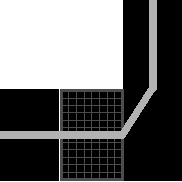
\includegraphics[width=0.1\textwidth]{symboly/kol1.png}
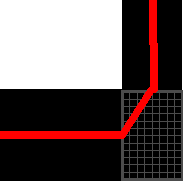
\includegraphics[width=0.1\textwidth]{symboly/kol2.png}
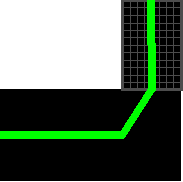
\includegraphics[width=0.1\textwidth]{symboly/kol3.png}
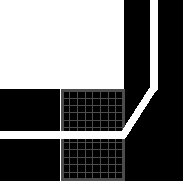
\includegraphics[width=0.1\textwidth]{symboly/kol4.png}
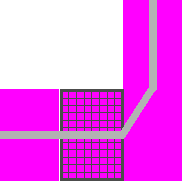
\includegraphics[width=0.1\textwidth]{symboly/kol22.png}
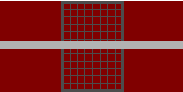
\includegraphics[width=0.1\textwidth]{symboly/kol8.png}

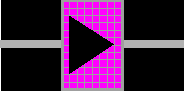
\includegraphics[width=0.1\textwidth]{symboly/hlnav16.png}
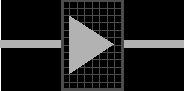
\includegraphics[width=0.1\textwidth]{symboly/hlnav1.png}
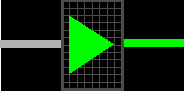
\includegraphics[width=0.1\textwidth]{symboly/hlnav2.png}
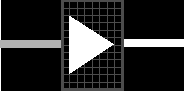
\includegraphics[width=0.1\textwidth]{symboly/hlnav3.png}
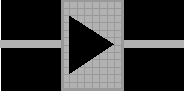
\includegraphics[width=0.1\textwidth]{symboly/hlnav5.png}
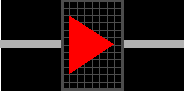
\includegraphics[width=0.1\textwidth]{symboly/hlnav6.png}
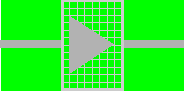
\includegraphics[width=0.1\textwidth]{symboly/hlnav8.png}

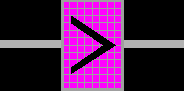
\includegraphics[width=0.1\textwidth]{symboly/senav6.png}
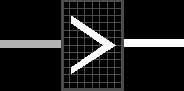
\includegraphics[width=0.1\textwidth]{symboly/senav2.png}
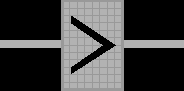
\includegraphics[width=0.1\textwidth]{symboly/senav3.png}
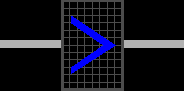
\includegraphics[width=0.1\textwidth]{symboly/senav4.png}

\includegraphics[width=0.1\textwidth]{symboly/senav8.png}

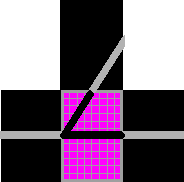
\includegraphics[width=0.1\textwidth]{symboly/vyh4.png}
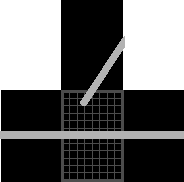
\includegraphics[width=0.1\textwidth]{symboly/vyh1.png}
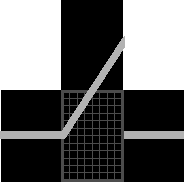
\includegraphics[width=0.1\textwidth]{symboly/vyh2.png}
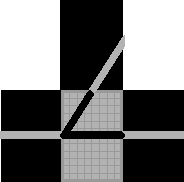
\includegraphics[width=0.1\textwidth]{symboly/vyh3.png}
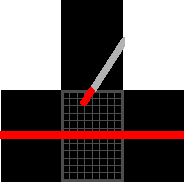
\includegraphics[width=0.1\textwidth]{symboly/vyh5.png}
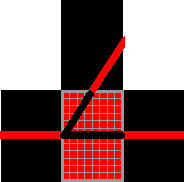
\includegraphics[width=0.1\textwidth]{symboly/vyh6.png}
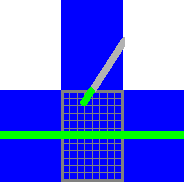
\includegraphics[width=0.1\textwidth]{symboly/vyh28.png}
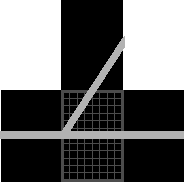
\includegraphics[width=0.1\textwidth]{symboly/vyh37.png}
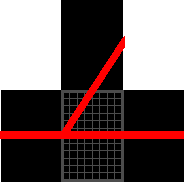
\includegraphics[width=0.1\textwidth]{symboly/vyh38.png}
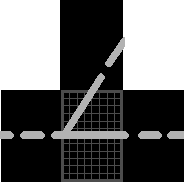
\includegraphics[width=0.1\textwidth]{symboly/vyh39.png}

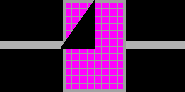
\includegraphics[width=0.1\textwidth]{symboly/vyk19.png}
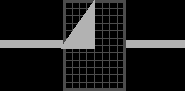
\includegraphics[width=0.1\textwidth]{symboly/vyk1.png}
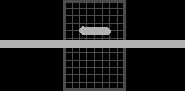
\includegraphics[width=0.1\textwidth]{symboly/vyk2.png}
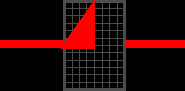
\includegraphics[width=0.1\textwidth]{symboly/vyk3.png}
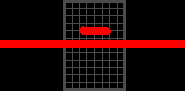
\includegraphics[width=0.1\textwidth]{symboly/vyk4.png}
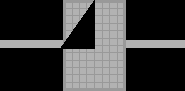
\includegraphics[width=0.1\textwidth]{symboly/vyk5.png}
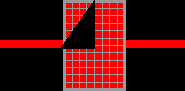
\includegraphics[width=0.1\textwidth]{symboly/vyk6.png}

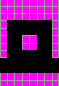
\includegraphics[width=0.05\textwidth]{symboly/ez6.png}

\includegraphics[width=0.05\textwidth]{symboly/ez1.png}

\includegraphics[width=0.05\textwidth]{symboly/ez2.png}
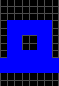
\includegraphics[width=0.05\textwidth]{symboly/ez3.png}
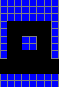
\includegraphics[width=0.05\textwidth]{symboly/ez5.png}

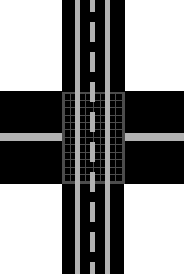
\includegraphics[width=0.1\textwidth]{symboly/prej1.png}
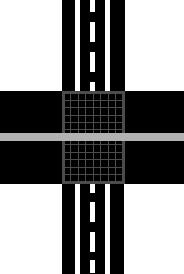
\includegraphics[width=0.1\textwidth]{symboly/prej2.png}
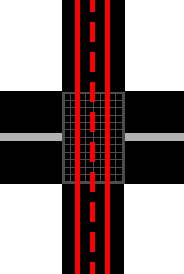
\includegraphics[width=0.1\textwidth]{symboly/prej3.png}

\item Kdy je a~kdy není nutné žádat o~traťový souhlas?
\solution{O~traťový souhlas není nutné žádat, pokud ho mám udělen, nebo pokud
jsem přihlášený do obou stanic tratě.}

\item Co je to závěr a k~čemu slouží?
\solution{Závěr je zapevnění bloku proti změně. Typicky například zamknutí
výhybky. Závěr se uděluje na bloky v jízdní cestě. Na výhybky, výkolejky a
úvazky lze ručně udělit nouzový závěr volbou \texttt{ZAV>} v~menu bloku.}

\item Sousední stanice mě žádá o~traťový souhlas, vy ho však chcete přijmout až
za minutu, jak nejlépe sdělit sousední stanici, že má počkat?
\solution{Napsat zprávu, zavolat, případně nechat žádost minutu pípat.
Zvuk žádosti lze dočasně potlačit klikem na ikonu v~horním panelu.}

\item Jak poznáte dopravní a~manipulační kolej?
\solution{Manipulační kolej je ohraničena seřaďovacími návěstidly. Pozor:
přerušovaný symbol koleje na reliéfu není manipulační kolej! Přerušovaný symbol
koleje na reliéfu je kolej bez indikace obsazení.}

\item Jak poznáte směr trati na reliéfu?
\solution{Ze směru šipky úvazky.}

\item Úvazka je červená, co to znamená?
\solution{Nastala porucha blokové podmínky trati.}

\end{enumerate}

\subsubsection*{Jízdní cesty}
\begin{enumerate}[leftmargin=*]
\item Má mít vlak v~ručním řízení postavenou jízdní cestu pro jízdu na
kolejišti?
\solution{Ano, vždy musí mít.}

\item Jak mohu zrušit jízdní cestu? Popište co nejvíce metod.
\solution{(a) Volbou \texttt{RC} na návěstidle, u~které začíná jízdní cesta
(JC). (b) Postupným nouzovým uvolněním závěrů (\texttt{NUZ}) všech úseků JC.
Závěr staniční koleje uvolňuje automaticky (neoznačuje se volbou \texttt{NUZ}).}

\item Popište vztah mezi pojmy \textit{jízdní cesta}, \textit{vlaková cesta}
a~\textit{posunová cesta}.
\solution{Jízdní cestou rozumíme cestu pro vlak (vlaková cesta) nebo pro posun
(posunová cesta).}

\end{enumerate}

\subsubsection*{Ruční řízení}
\begin{enumerate}[leftmargin=*]
\item Vyjmenujte všechny možnosti, jak řídit lokomotivu ručně.
\solution{(a) Skrze aplikaci Jerry. (b) Skrze aplikaci hJOPdriver. (c) Pomocí
Roco Multimaus a~uLI.}

\item Co znamená, když je v~ovladači zaškrtnuto \textit{ruční řízení}
a k~čemu vás to opravňuje?
\solution{\textit{Ruční řízení} znamená, že řídíte jízdu vlaku.}

\end{enumerate}

\subsubsection*{Krizové scénáře}
\begin{enumerate}[leftmargin=*]
\item Jako posunovač máte volnou chvíli, ohlédnete se do sousední stanice
a~vidíte, že dva vlaky jedou proti sobě a~nezpomalují, přibližně za 5 s~do sebe
narazí. Co uděláte?
\solution{Klik na červenou ikonku na horní liště panelu \textit{Zastavit DCC
na celém kolejišti}. Poté otevřít ovladač obou souprav, zastavit je a pustit
DCC. Tím lokomotivy zůstanou stát a~celé kolejiště se rozjede.}

\item Kdy použít nouzové zastavení celého kolejiště a~kdy vybrané soupravy?
\solution{Nouzové zastavení celého kolejiště používejte v~případě, kdy není
možné vlak zastavit jinak. Typicky například proto, že se vlak nenachází
v~obvodu vámi řízené stanice. Nouzové zastavení celého kolejiště je krajní
volbou!}

\end{enumerate}

\subsubsection*{Odpovědnost}
\begin{enumerate}[leftmargin=*]
\item Popište, za co jako dispečer odpovídáte.
\solution{Za všechny soupravy v~obvodu vámi řízených stanic – za to, že se
nepoškodí.}

\item Co dělat, když na kolejišti něco rozbijete?
\solution{Nahlásit starší obsluze.}

\end{enumerate}

\subsubsection*{Vlakotvorba}
\begin{enumerate}[leftmargin=*]
\item Popište, podle čeho se rozhodujete jaký vlak kdy a kam poslat.

\item Kde se dozvíte, co stanice vyváží a dováží?
\solution{Na každé stanici je výtisk datových listů. Dostupné také online:\\
\url{https://github.com/kmzbrnoI/ds-tt/releases}}.

\item Které úkony je nutné vykonat k~řádnému zpracování manipulačního vlaku,
který vám právě přijel do stanice? Zpracování manipulačního vlaku končí
v~momentě jeho odjezdu ze stanice.
\solution{V~editaci vlaku je v~poznámce k~soupravě uvedeno, jak naložit
s~jednotlivými vagony. Vyřešit požadavky, které se týkají aktuální stanice.
Přidat do soupravy vagony dle poptávky a plánů. Upravit počet vozů, délku
vlaku a popis vagónů dle změn.}

\item Potřebujete lokomotivní zálohu z~výtopny/depa, jak ji získáte?
\solution{Zavoláte/napíšete do depa a~zálohu si vyžádáte.}

\item Co to znamená, že se na kolejišti \textit{jezdí nákladní doprava} a~jak
nákladní doprava funguje?

\item Kam píšete nákladní vozy ve vlaku?
\solution{V~editaci vlaku do pole \textit{Poznámky} k~soupravě.}

\end{enumerate}

\subsubsection*{Další}
\begin{enumerate}[leftmargin=*]
\item Co je to riziková funkce?
\solution{Jedná se o~rizikové operace, jako například rušení vlaku,
přestavování obsazené výhybky, uvolňování závěru. Při průběhu rizikové funkce
je zobrazeno speciální okno, kde je třeba operaci ještě jednou potvrdit.}

\item Které všechny úkony je nutné vykonat při potvrzování rizikové funkce?
Uveďte na příkladu nouzového stavění výhybky.
\solution{Je nutné přečíst si potvrzovanou rizikovou funkci a výpis
kontrolovaných podmínek. Občas se ve výpisu může objevit čekání na nějakou
akci (uzavření přejezdu / přestavení výhybky), v~takovém případě je nutné
počkat na dokončení těchto úkonů. A~poté odsouhlasit seznam kontrolovaných
podmínek.}

\end{enumerate}


\newpage
\section{S1u – dispečer řízení jízdy přes uLI}

Musí být součástí zaškolení úrovně S1 pro kolejiště, kde se používají
uLI-daemon.

\subsection{Praktická část}

\begin{enumerate}[leftmargin=*]
\item Proveďte převzetí, řízení a uvolnění soupravy na Roco Multimaus.
\end{enumerate}

\subsection{Teoretická část}

\begin{enumerate}[leftmargin=*]

\item Co je to \textit{uLI-daemon} a~jakou má funkci?
\solution{Je to aplikace umožňující funkci uLI-master. Spouští se se startem
prvního panelu na dispečerském počítači, při nechtěném ukončení lze znovu
zapnout ikonkou na horní liště panelu.}

\item Co je to \textit{uLI-master} a~jakou má funkci?
\solution{Je to černá krabička rozměru 7×5 cm, umožňující připojení Roco
Multimaus k~počítači se spuštěným panelem a uLI-daemonem.}

\item Ikonka mašinky na Rocomaus bliká, co to znamená?
\solution{Multimaus neovládá žádnou lokomotivu.}

\item Ikonka mašinky na Rocomaus trvale svítí, mašinka přesto nereaguje,
co je špatně?
\solution{Může to znamenat, že není zaškrtnuto \textit{Ruční řízení} (tedy, že
ovládáte pouze funkce a~nikoliv jízdu) nebo lokomotiva/y uvízla na špíně nebo
jste na ovladač přidělili špatnou lokomotivu/y.}

\end{enumerate}


\newpage
\section{S2 – pokročilý dispečer}

Opravňuje k~řízení větších stanic. Obsahuje otázky na veškerou funkcionalitu,
kterou umí hJOP nabídnout.

\subsection{Praktická část}

\begin{enumerate}[leftmargin=*]
\item Demonstrujte zapnutí a~vypnutí kolejiště a~serveru.
\item Rozsviťte přivolávací návěst na návěstidle bez postavení nouzové cesty.
\item Proveďte příjem vlaku na obsazenou kolej včetně zrušení nouzové cesty.
\item Ručně uzavřete přejezd.
\item Proveďte nouzové otevření přejezdu.
\item Vytvořte a zrušte soupravu s~více lokomotivami.
\item Přidejte na kolej více souprav.
\item Přesuňte soupravu na jinou kolej.
\item Prohoďte soupravy na jedné koleji.
\item Proveďte vytvoření nové lokomotivy.
\item Proveďte úpravu dat lokomotivy.
\item Zjistěte, kde se nachází lokomotiva s~danou adresou.
\item Nastavte modelový čas, zapněte jej a vypněte jej.
\item Předveďte práci se zásobníkem povelů: přidání povelu, pozastavení
zásobníku, smazání povelu, přesun povelů.
\item Proveďte maximálně možně zabezpečený nouzový vjezd vlaku na manipulační
kolej.
\item Demonstrujte multitrakci v~ručním ovladači.
\item Zaveďte předvídaný odjezd vlaku.
\item Zaveďte na návěstidle režim AB, zrušte režim AB.
\item Postavte JC s~variantními body.
\item Postavte složenou JC s~variantními body.
\end{enumerate}

\newpage
\subsection{Teoretická část}

\begin{enumerate}[leftmargin=*]
\item Vysvětlete význam náslědujících symbolů. \\
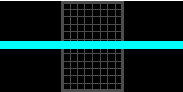
\includegraphics[width=0.1\textwidth]{symboly/kol5.png}
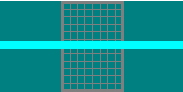
\includegraphics[width=0.1\textwidth]{symboly/kol7.png}
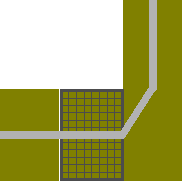
\includegraphics[width=0.1\textwidth]{symboly/kol20.png}
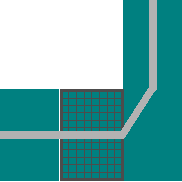
\includegraphics[width=0.1\textwidth]{symboly/kol21.png}

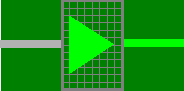
\includegraphics[width=0.1\textwidth]{symboly/hlnav9.png}
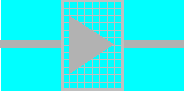
\includegraphics[width=0.1\textwidth]{symboly/hlnav15.png}
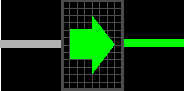
\includegraphics[width=0.1\textwidth]{symboly/hlnav17.png}
\includegraphics[width=0.1\textwidth]{symboly/hlnav18.png}
\includegraphics[width=0.1\textwidth]{symboly/hlnav19.png}
\includegraphics[width=0.1\textwidth]{symboly/senav14.png}

\includegraphics[width=0.1\textwidth]{symboly/vyh7.png}
\includegraphics[width=0.1\textwidth]{symboly/vyh8.png}
\includegraphics[width=0.1\textwidth]{symboly/vyh14.png}
\includegraphics[width=0.1\textwidth]{symboly/vyh21.png}
\includegraphics[width=0.1\textwidth]{symboly/vyh22.png}
\includegraphics[width=0.1\textwidth]{symboly/vyh23.png}
\includegraphics[width=0.1\textwidth]{symboly/vyh24.png}
\includegraphics[width=0.1\textwidth]{symboly/vyh25.png}
\includegraphics[width=0.1\textwidth]{symboly/vyh26.png}
\includegraphics[width=0.1\textwidth]{symboly/vyh27.png}

\includegraphics[width=0.1\textwidth]{symboly/vyk9.png}
\includegraphics[width=0.1\textwidth]{symboly/vyk10.png}
\includegraphics[width=0.1\textwidth]{symboly/vyk11.png}
\includegraphics[width=0.1\textwidth]{symboly/vyk17.png}

\includegraphics[width=0.05\textwidth]{symboly/ez4.png}

\item Nouzové závěry kterých bloků se automaticky neruší při volbě \textit{RNZ
– rušení nouzových závěrů} a~je třeba je zrušit ručně?
\solution{Závěr trati, uzavření přejezdu, závěr zámků.}

\item Jaké všechny povely lze vkládat do zásobníku povelů?
\solution{Stavění jízdní cesty (vlakové i~posunové cesty), žádost o~traťový
souhlas, udělení traťového souhlasu.}

\item Zásobník povelů je přepnutý do volby \textit{PV}, je zásobník aktivní?
\solution{Ne. Dočasné přepnutí zásobníku do volby \textit{PV} se používá
k~dočasnému pozastavení funkce zásobníku, například při nutnosti aktuálně
vykonat prioritní povel.}

\item Mohu vypnout napájecí zdroj stanice za plného provozu? Co po vypnutí
napájení udělá ovládací panel?
\solution{Ano, je to možné, ale zastaví to provoz v~celém napájeném úseku.
Symboly na reliéfu zfialoví.}

\item Mohu při restartu hJOP nechat vlaky v~trati?
\solution{Ano, vlaky můžou zůstat kdekoliv. Při běžné vypínání kolejiště se
doporučuje dojet do stanic.}

\item Na jaké úseky lze a~na jaké nelze přesouvat vlaky?
\solution{Vlaky lze přesouvat na staniční koleje a~některé vlečky. Na zbylé
úseky (zhlaví,  záhlaví, trať, ...) soupravy přesouvat nelze.}

\item Vysvětlete barvy soupravy předvídaného odjezdu vlaku.

\item Vysvětlete chování režimu AB u~návěstidla.

\end{enumerate}

\end{document}
